\documentclass[11pt]{article}
\usepackage{fullpage}
\usepackage{graphicx}
\usepackage{amsmath}
\usepackage{amssymb}
\usepackage{amsthm}
\usepackage{algorithm}
\usepackage{algorithmic}
\usepackage{float}
%\setlength{\hoffset}{-1.0cm}
%\setlength{\voffset}{-1.0cm}
%\setlength{\textheight}{8.5in}
%\setlength{\textwidth}{6.0in}

% Some utilities

\newcommand{\comment}[1]{}
\newenvironment{definition}[1][Definition]{\begin{trivlist}
\item[\hskip \labelsep {\bfseries #1}]}{\end{trivlist}}
\newenvironment{remark}[1][Remark]{\begin{trivlist}
\item[\hskip \labelsep {\bfseries #1}]}{\end{trivlist}}
\newtheorem{theorem}{Theorem}[section]
\newtheorem{lemma}[theorem]{Lemma}

\title{Design and Display of Rational B-spline Motion with the Global Least Squares Approximation and Interpolation Motion Techniques}
\author{ Steven Zilg, Austin Henthorne }
\date{\today}

\begin{document}

\begin{titlepage}
\centering
\LARGE{\textbf{Design and Display of Rational B-spline Motion with the Global Least Squares Approximation and Interpolation Motion Techniques}}

\vspace{2cm}
\Large{Authors:}

\Large{Austin Henthorne}

\Large{Steven Zilg}

\vfill

\Large{Stony Brook University}

\Large{ MEC 572}

\Large{\today}
\end{titlepage}

\newpage
\section{Introduction}

Motion control is inherently important throughout engineering, ranging from theoretical modeling to physical mechanism construction. Particularly during the age of robotics and artificial intelligence, research is constantly being conducted to ensure the motion of robots and robotic mechanisms can be optimised. B-splines and dual quaternions have historically been important tools in the fields of path analysis and motion generation. This paper will demonstrate an alternative method in which these tools can be used together to generate meaningful object motion.

\newpage
\section{Background Research}

\textbf{\large{B-spline}}
\\
A non-rational B-spline curve is derived from the bezier curve but unlike the bezier, the degree of the B-spline curve is independent of the number of control points which makes this curve more desirable. The B-spline curve is dependent on the control points, control functions, the degree, and the knot vector (Piegl and Tiller, 1995). The equation of the B-spline is as follows:
$$P(u) = \sum^n_{i=0} N_{i,p}(u)P_i, \qquad u_{min}\leq u < u_{max}$$
The $N_{i,p}$ represents the basis function of control point $P_i$.
$$N_{i,0}(u) = \left\{
                 \begin{array}{ll}
                   1, & \hbox{$u_i \leq u < u_{i+1}$} \\
                   0, & \hbox{otherwise}
                 \end{array}
               \right.$$
$$ N_{i,p} = \frac{u-u_i}{u_{i+p}-u_i} N_{i,p-1}(u)+ \frac{u_{i+p+1}-u}{u_{i+p+1}-u_{i+1}} N_{i+1,p-1}(u)$$
Thus, changing the control points, the knots, or the degree of the curve will change the shape of the B-spline curve.
\\
\\
A non-uniform rational B-spline (NURBS) curve introduces a concept called weights which gives the user more control of manipulating a curve. Each weight corresponds to a multiplier for a respective control point, and changing the weight will make the curve pass arbitrarily far or near to a control point. The piecewise rational B-spline curve is defined as:
$$ P(u) = \frac{\sum^n_{i=0} \omega_i P_i N_{i,p}(u)}{\sum^n_{i=0} \omega_i N_{i,p}(u)}, \qquad u_{min} \leq u < u_{max} $$
\\
For this report and software implementation, weights for all points will be set to 1 so that the generic NURBS form reduces to the non-rational equation stated above. Additionally, all knot vectors will be designed for clamped B-spline behavior, to ensure all curves travel through the desired starting and ending points.
\\
\\
\textbf{\large{Approximation/Interpolation}}
\\
To develop NURBS curves that fit an arbitrary set of data points we had to study interpolation and approximation. A curve that satisfies interpolation will go through each point precisely. Unlike interpolation, approximation will not go through each point but will only approximate the data points. With approximation it is important to capture the shape of the data, but with interpolation it is essential to exactly represent a curve that will pass though each point (Piegl and Tiller, 1995).
\\
\\
\textbf{Global Curve Interpolation:}
\\
Suppose we would like to interpolate a given set of data points denoted as $\{Q_k\}, k = 0,\ldots,n$ with a $p$th-degree B-spline curve. The parameter value will be given as $\bar{u}_k$ for each $\{Q_k\}$ and we select a proper knot vector $U = \{u_0,\ldots,u_m\}$, $u \in [0,1]$.
\\
$$Q_k = C(\bar{u}_k) = \sum^n_{i=0}N_{i,p}(\bar{u}_k)P_i$$
The unknowns in this equation are the $n+1$ control points, $P_i$. To solve for the control points,  we set up $(n+1) \times (n+1)$ system of linear equations. Three common methods for choosing the  parameter value $(\bar{u}_k)$ are equally spaced, chord length and the centripetal method.
\begin{itemize}
  \item Equally Spaced:
  \\
  $$ \bar{u}_0 = 0 \qquad \bar{u}_n = 1 $$
  $$ \bar{u}_k = \frac{k}{n} \qquad k = 1,\ldots,n-1$$
  When the data is unevenly spaced, this method could produce unpredictable shapes such as loops.
  \item Chord length:
  \\
  d = total chord length
  $$ d = \sum^n_{k=1} |Q_k-Q_{k-1}|$$
  With: \qquad $ \bar{u}_0 = 0 \qquad \bar{u}_n = 1 $
  $$ \bar{u}_k = \bar{u}_{k-1} + \frac{|Q_k-Q_{k-1}|}{d} \qquad k = 1,\ldots, n-1$$
  This is a commonly used method since it gives a good parameterization to the curve.
  \item Centripetal:
  \\
  $$ d = \sum^n_{k=1} \sqrt{|Q_k-Q_{k-1}|}$$
  With: \qquad $ \bar{u}_0 = 0 \qquad \bar{u}_n = 1 $
  $$ \bar{u}_k = \bar{u}_{k-1} + \frac{\sqrt{|Q_k-Q_{k-1}|}}{d} \qquad k = 1,\ldots, n-1$$
  This method gives better results than the chord length when the data takes sharp turns.
\end{itemize}
Two common methods for selecting knots are equally spaced and another technique called averaging (Piegl and Tiller, 1995).
\begin{itemize}
  \item Equally Spaced:
  \\
  $$ u_0 = \ldots = u_p = 0 \qquad u_{m-p} = \ldots = u_m = 1$$
  $$ u_{j+p} = \frac{j}{n-p+1} \qquad j = 1,\ldots, n-p$$
  This method is not recommended because of a result in a singular system of equations if used in conjunction with chord length or centripetal method for parameter values.
  \item Averaging:
  \\
  $$ u_0 = \ldots = u_p = 0 \qquad u_{m-p} = \ldots = u_m = 1$$
  $$ u_{j+p} = \frac{1}{p} \sum^{j+p+1}_{i=j} \bar{u}_i \qquad j = 1,\ldots,n-p$$
  This method best reflects the knots with the distribution of the parameter values.
\end{itemize}
Once the parameters and knot values are finalized, the basis functions $N_{i,p}(u)$ can be calculated for each data point. Because each data point results from a linear combination of the unknown control points, the solution for the control points reduces to a simple system of linear equations with cofficient matrix

$$N = \left[\begin{array}{ccc}
  N_{0,p}(\bar{u}_0) & \ldots & N_{n,p}(\bar{u}_0) \\
   \vdots& \ddots & \vdots \\
  N_{0,p}(\bar{u}_{n}) & \ldots & N_{n,p}(\bar{u}_{n})
\end{array}\right]$$
\\
The unknowns $P_i$ in the equation $C(\bar{u}_k) = NP_i$ can be solved for by $P_i = N^TC(\bar{u}_k)$.
\\
\\
\textbf{Least Squares Curve Approximation:}
\\
A similar analysis can be performed for curve approximation of $m+1$ data points using $n+1$ control points. We analyze a B-spline curve with a $p$th degree. The knots and parameters are also precalculated using one of the methods listed in global interpolation (Piegl and Tiller, 1995). We assume $p\geq 1, n\geq p$ and $Q_0 = C(0)$ and $Q_m = C(1)$:
$$ C(u) = \sum^n_{i=0} N_{i,p}(u)P_i \qquad u \in [0,1]$$
Using least squares the remaining $Q_k$ are approximated:
$$ \sum^{m-1}_{k=1} |Q_k - C(\bar{u}_k)|^2$$
$$ R_k = Q_k - N_{0,p}(\bar{u}_k)Q_0 - N_{n,p}(\bar{u}_k)Q_m \qquad k=1,\ldots, m-1$$
$f$ is a scalar-valued function of the n-1 variables, $P_1,\ldots, P_{n-1}$:
$$ f = \sum^{m-1}_{k=1} |Q_k - C(\bar{u}_k)|^2 = \sum^{m-1}_{k=1} |R_k - \sum^{n-1}_{i=1} N_{i,p}(\bar{u}_k) P_i |^2$$
$$= \sum^{m-1}_{k=1} \bigg[R_k\cdot R_k - 2\sum^{n-1}_{i=1} N_{i,p}(\bar{u}_k)(R_k\cdot P_i) + \bigg(\sum^{n-1}_{i=1} N_{i,p}(\bar{u}_k)P_i \bigg) \cdot \bigg(\sum^{n-1}_{i=1}N_{i,p}(\bar{u}_k)P_i \bigg) \bigg]$$
Appling least squares fitting, to minimize $f$ we set the derivatives of $f$ with respect to the $n-1$ points, $P_\ell$, equal to zero. The partial derivative with respect to the $\ell$th control point is:
$$\frac{\partial f}{\partial P_\ell} = \sum^{m-1}_{k=1} \bigg(-2N_{\ell,p}(\bar{u}_k)R_k + 2N_{\ell,p}(\bar{u}_k)\sum^{n-1}_{i=1}N_{i,p}(\bar{u}_k)P_i \bigg)$$
which implies;
$$ -\sum^{m-1}_{k=1}N_{\ell,p}(\bar{u}_k)R_k + \sum^{m-1}_{k=1} \sum^{n-1}_{i=1}N_{\ell,p}(\bar{u}_k)N_{i,p}(\bar{u}_k)P_i = 0$$
It follows;
$$ \sum^{n-1}_{i=1} \bigg(\sum^{m-1}_{k=1} N_{\ell,p}(\bar{u}_k) N_{i,p}(\bar{u}_k) \bigg)P_i = \sum^{m-1}_{k=1}N_{\ell,p}(\bar{u}_k)R_k$$
The above equation results in a linear system with only the control points $P_1,\ldots,P_{n-1}$ as the unknowns. With $\ell=1,\ldots,n-1$ returns the system of $n-1$ equations in $n-1$ unknowns:
$$(N^T N)P = R$$
Where N is the $(m+1)\times(n+1)$ matrix of scalars:
$$N = \left[\begin{array}{ccc}
  N_{0,p}(\bar{u}_0) & \ldots & N_{n,p}(\bar{u}_0) \\
   \vdots& \ddots & \vdots \\
  N_{0,p}(\bar{u}_{m}) & \ldots & N_{n,p}(\bar{u}_{m})
\end{array}\right]$$

R is the vector of $n+1$ points:
$$R =N^TQ_k= \left[\begin{array}{c}
    N_{0,p}(\bar{u}_0)Q_0+\ldots+N_{0,p}(\bar{u}_{m})Q_{m} \\
    \vdots \\
    N_{n,p}(\bar{u}_0)Q_0+\ldots+N_{n,p}(\bar{u}_{m})Q_{m}
  \end{array}\right]$$
The control points:
$$ P = \left[\begin{array}{c}
         P_0 \\
         \vdots \\
         P_{n}
       \end{array}\right]$$
\\
\\
\textbf{\large{B-spline Motion}}
\\
The dual quaternion representation of spatial displacement has recently dominated the realm of motion. Many people are familiar with the 4x4 matrix representation of rigid body transformation but they are computationally inefficient as they include 16 numbers for one spatial displacement. Dual quaternions represent the same spatial displacement as the matrices but only consist of 8 elements. The advantages of dual quaternion is that they are a very neat, compact way of expressing spatial displacement and that they have been proven to be an efficient and practical method for interpolation in three-dimensional motions. The B-spline motion equation is identical to the previous equation stated but the curve $\hat{Q}(t)$ and the control points $\hat{Q}_i$ will be expressed as dual quaternions:
$$ \hat{Q}(t) = \sum^n_{i=0} N_{i,p} \hat{Q}_i$$
\\
The proposed method of polar decomposition seeks to improve on this method of B-spline motion generation.
\\
\textbf{Polar Decomposition of Unit Dual Quaternions:}
\\
One primary concern with the dual quaternion representation of spatial displacement is the idea of interpolating between dual quaternions. A given dual quaternion has both a real part with rotational units and a dual part with translational units of length. Because of this, there is often a debate over the meaning of subtracting two spatial displacements, and subsequently interpolating between them. In this section we convert a unit dual quaternion representation of a spatial displacement into a double quaternion. A double quaternion is a pair of quaternions that serves to approximate a dual quaternion, thus making the difference between two spatial displacements entirely rotational (Purwar and Ge, 2013).
\\
\\
Let a unit dual quaternion be denoted as: $$\hat{\textbf{Q}} = \textbf{Q} + \epsilon\textbf{Q}^0$$
\\
Where \textbf{Q} is the real part that represents a 3D rotation.
\\
The dual part $\textbf{Q}^0$ is derived from the translation vector \textbf{d}, and the real part \textbf{Q}:
\\
$$ \textbf{Q}^0 = \frac{1}{2}\textbf{d}\textbf{Q}$$
Let $\epsilon = \frac{1}{R}$, Where $R = \frac{24L}{\pi}$ and $L$ is the largest translation element in all the given displacements.
$$\hat{\textbf{Q}} = \textbf{Q} + \epsilon\textbf{Q}^0 = \hat{\textbf{Q}} + \frac{1}{2R}\textbf{d}\textbf{Q} = (1+\frac{d}{2R}\bar{\textbf{d}})\textbf{Q} = r\textbf{D\textbf{Q}}$$
Where $ r = \frac{\sqrt{4R^2+d^2}}{2R}$, and \textbf{D} is a unit quaternion denoted as:
$$\textbf{D} = \frac{2R}{\sqrt{4R^2+d^2}}+\bar{\textbf{d}}\frac{d}{\sqrt{4R^2+d^2}}$$
Similarly,
$$\hat{\textbf{Q}} = \textbf{Q} - \epsilon\textbf{Q}^0 = \hat{\textbf{Q}} - \frac{1}{2R}\textbf{d}\textbf{Q} = (1-\frac{d}{2R}\bar{\textbf{d}})\textbf{Q} = r\textbf{D}^\ast\textbf{Q}$$
\\
This gives us a pair of unit quaternions, \textbf{G} and \textbf{H}
$$ \textbf{G} = \textbf{D}\textbf{Q} \qquad \textbf{H} = \textbf{D}^\ast\textbf{Q}$$
Thus,
$$\textbf{Q}+\epsilon\textbf{Q}^0 = r\textbf{G} \qquad \textbf{Q}-\epsilon\textbf{Q}^0 = r\textbf{H}$$
\textbf{G} and \textbf{H} together represent a double quaternion pair. For any such pair, the above steps can be reversed to obtain a corresponding dual quaternion and spatial displacement. Using this method, interpolation or approximation can be performed using \textbf{G} and \textbf{H}, such that the distance between data points can be entirely measured in radians. The results of this method are dependent on $R$, the radius of the proposed hypersphere used to approximate the linear translation as a rotation. This paper will demonstrate that if $R$ is sufficiently large (Larochelle and McCarthy, 1994), the results of this method will be consistent with a B-spline interpolation or approximation on the dual quaternions themselves.
\\
\\
\newpage
\section{Implementation}
In this paper we set out to accomplish three tasks:
\begin{enumerate}
  \item Create rational B-spline motion using the configuration inputs as control points.
  \item Generate interpolation motion using a rational B-spline curve.
  \item Produce approximation motion using a rational B-spline curve.
\end{enumerate}
We utilized the Microsoft Visual Studio software to code our implementation in C++. We converted our code into a executable file format to allow any Windows platform to run our program. The user will have the option to upload a file containing a spatial description of a rigid body displacement in 3D space. This spatial description will include a rotation component expressed as a quaternion, and a translation part of four elements with the first three elements as the x-y-z coordinates and the last element as zero. Our program has a default number of four spatial displacements spread out randomly in space.  An arbitrary number of rigid body displacements is allowed for the user input.
\\
\\
\textbf{\large{B-spline}}
\\
To obtain a rational B-spline motion we simply started with the governing equation:
$$ P(u) = \frac{\sum^n_{i=0} \omega_i P_i N_{i,p}(u)}{\sum^n_{i=0} \omega_i N_{i,p}(u)}$$
We replaced the control points and the curve components with dual quaternions:
$$ Q(u) = \frac{\sum^n_{i=0} \omega_i Q_i N_{i,p}(u)}{\sum^n_{i=0} \omega_i N_{i,p}(u)}$$
With both the $Q(u)$ representing the rational B-spline curve and $Q_i$ denoting the control points as dual quaternions.
\\
\\
We derive the control points $Q_i$ from the user input. Let the control points be expressed as:
$$ Q_i = Q_r + \epsilon Q_t $$
We obtain the quaternion $Q_r$ directly from the users input for the rotation part of the spatial displacement. The dual part of the dual quaternion $Q_t$ is derived from both of the users input of the translation vector and the real part $Q_r$:
$$ Q_t = \frac{1}{2}t Q_r $$
With $t$ = translation vector, and noting that $tQ_r$ is a quaternion multiplication.
\\
\\
To solve for the knot vector we employ equally spaced method to obtain the knots:
$$ u_0 = \ldots = u_p = 0 \qquad u_{m-i} = 1 \qquad i = 0,\ldots , p$$
$$ u_{i+p} = \frac{i}{m} \qquad i = 0,\ldots, m$$
Where $p$ = degree, $m$ = (number of positions) + $p$
\\
\\
Next we solve for the basis function using the knots:
$$ N_{i,p}(u) = \frac{u-u_i}{u_{i+s}-u_i} N_{i,p-1}(u)+ \frac{u_{i+s+1}-u}{u_{i+s+1}-u_{i+1}} N_{i+1,p-1}(u)$$
$$ u = \frac{z}{r} \qquad z = 0,\ldots , r \qquad s = 1,\ldots , p \qquad i = 0,\ldots , m-s-1 $$
Where $r$ is the resolution i.e; the number of positions between all displacements.
\\
\\
Finally we set all the weights equal to one, $\omega = 1$, as previously stated.
\\
\\
With all the elements of the rational B-spline equation accounted for, we convert the dual quaternion equation into a homogeneous matrix and output the result. Overall the user input for this function is the degree and the resolution, as well as the control points themselves. Figure 1 shows an adequate expression of a second degree rational B-spline curve generated with the above algorithm.
\\
\\
\begin{figure}[h]
  \centering
  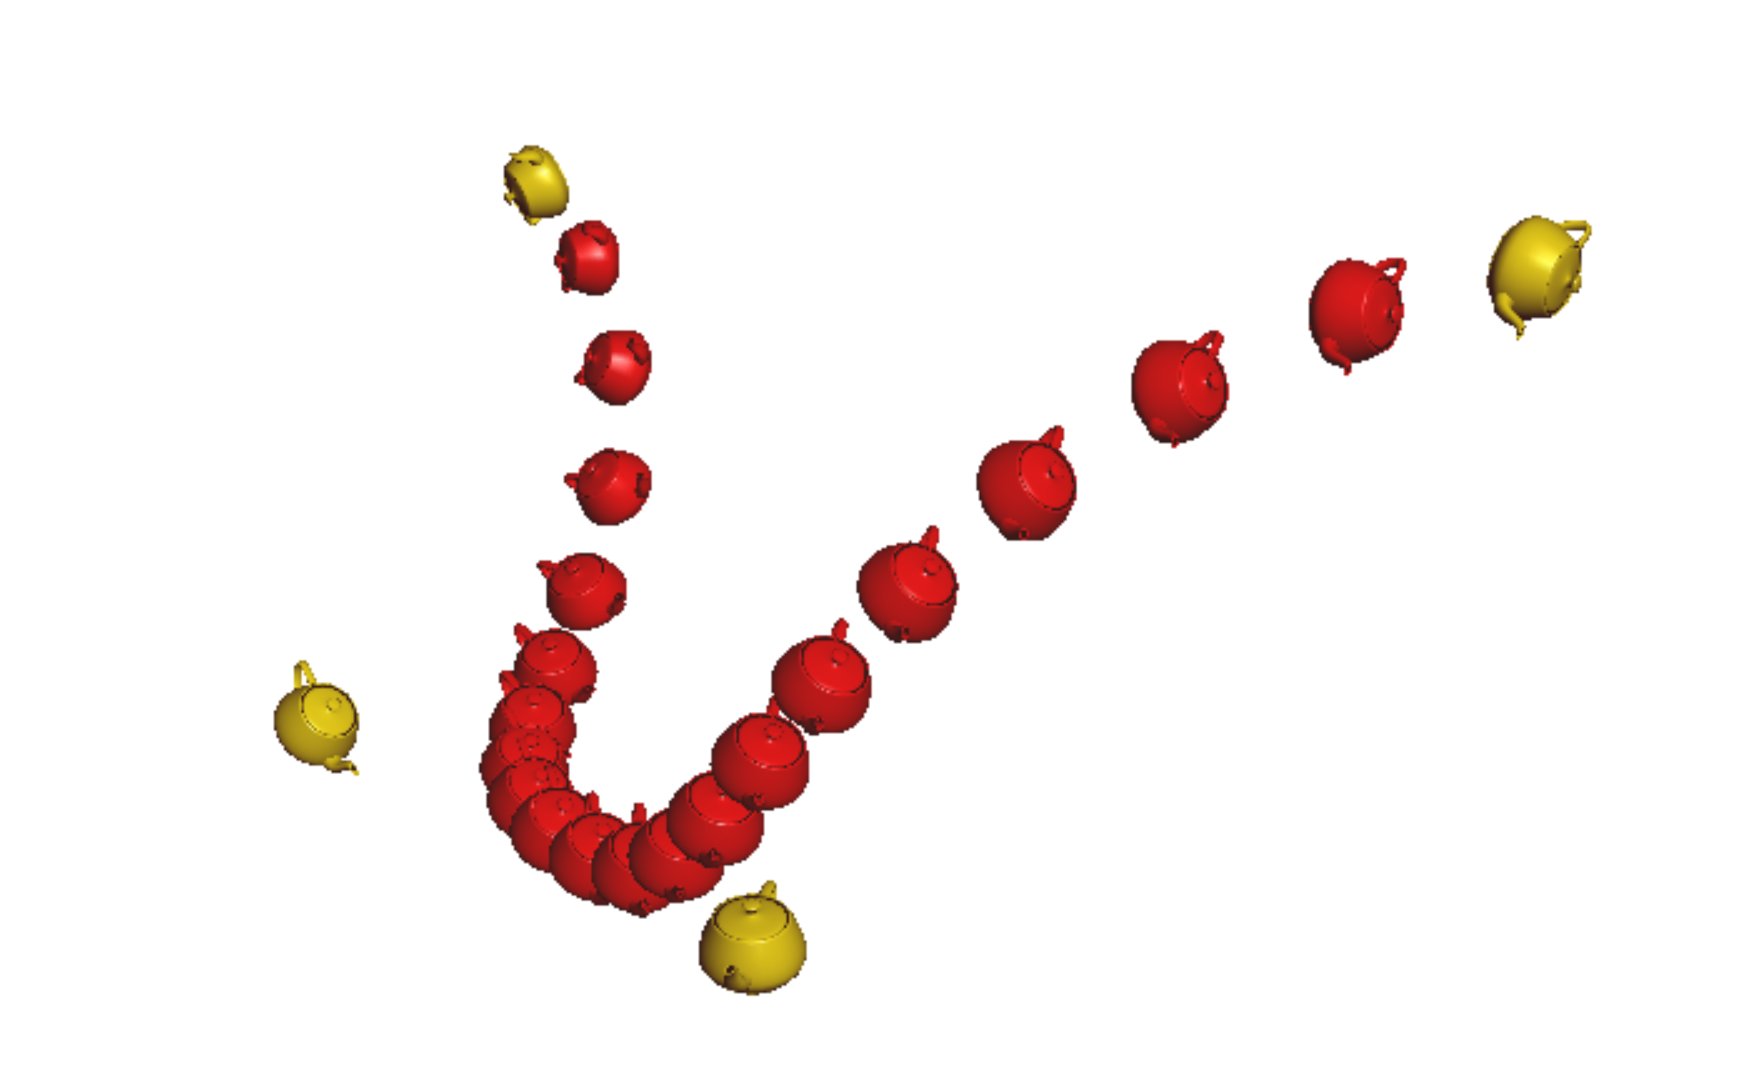
\includegraphics[width=0.75\textwidth]{B-spline.png}
  \caption{Degree 2 B-spline curve generated using the data points as control points.}
  \label{Figure: 1}
\end{figure}
\\
\textbf{\large{Interpolation/Approximation Using Dual Quaternions}}
\\
Because the solutions to interpolation and approximation are similar, our implementation handles both solutions using the same algorithm, where the user can select the desired number of control points the resulting curve should implement. If the number of desired control points are equal to the number of data points, we obtain an interpolation curve. If the number of control points do not equal to the number of data points, we acquire an approximation curve. The following is our method for solving for the required control points themselves.
\\
\\
We first calculate our parameters, $\bar{u}_k$, using the equally spaced method:
$$ \bar{u}_0 = 0 \qquad \bar{u}_n = 1 $$
$$ \bar{u}_k = \frac{k}{n} \qquad k = 1,\ldots,n-1$$
Where $n+1$ is the number of positions.
\\
\\
The knots are computed just like before using the equally spaced method:
$$ u_0 = \ldots = u_p = 0 \qquad u_{m-i} = 1 \qquad i = 0,\ldots , p$$
$$ u_{i+p} = \frac{i}{m} \qquad i = 0,\ldots, m$$
$p$ = degree, $m$ = $c$ + $p$
\\
Where $c$ is the user controlled number of control points. These methods are used to simplify the algorithm so that it can be used for both interpolation as well as approximation generations.
\\
\\
Next we solve for $N_{i,p}(\bar{u}_k)$:
$$ N_{i,p}(\bar{u}_k) = \frac{\bar{u}_k-u_i}{u_{i+s}-u_i} N_{i,p-1}(\bar{u}_k)+ \frac{u_{i+s+1}-\bar{u}_k}{u_{i+s+1}-u_{i+1}} N_{i+1,p-1}(\bar{u}_k) $$
$$ i = 0,\ldots, m-s-1 \qquad s = 1,\ldots, p \qquad k = 0,\ldots, n-1 $$
\\
\begin{figure}[h]
  \centering
  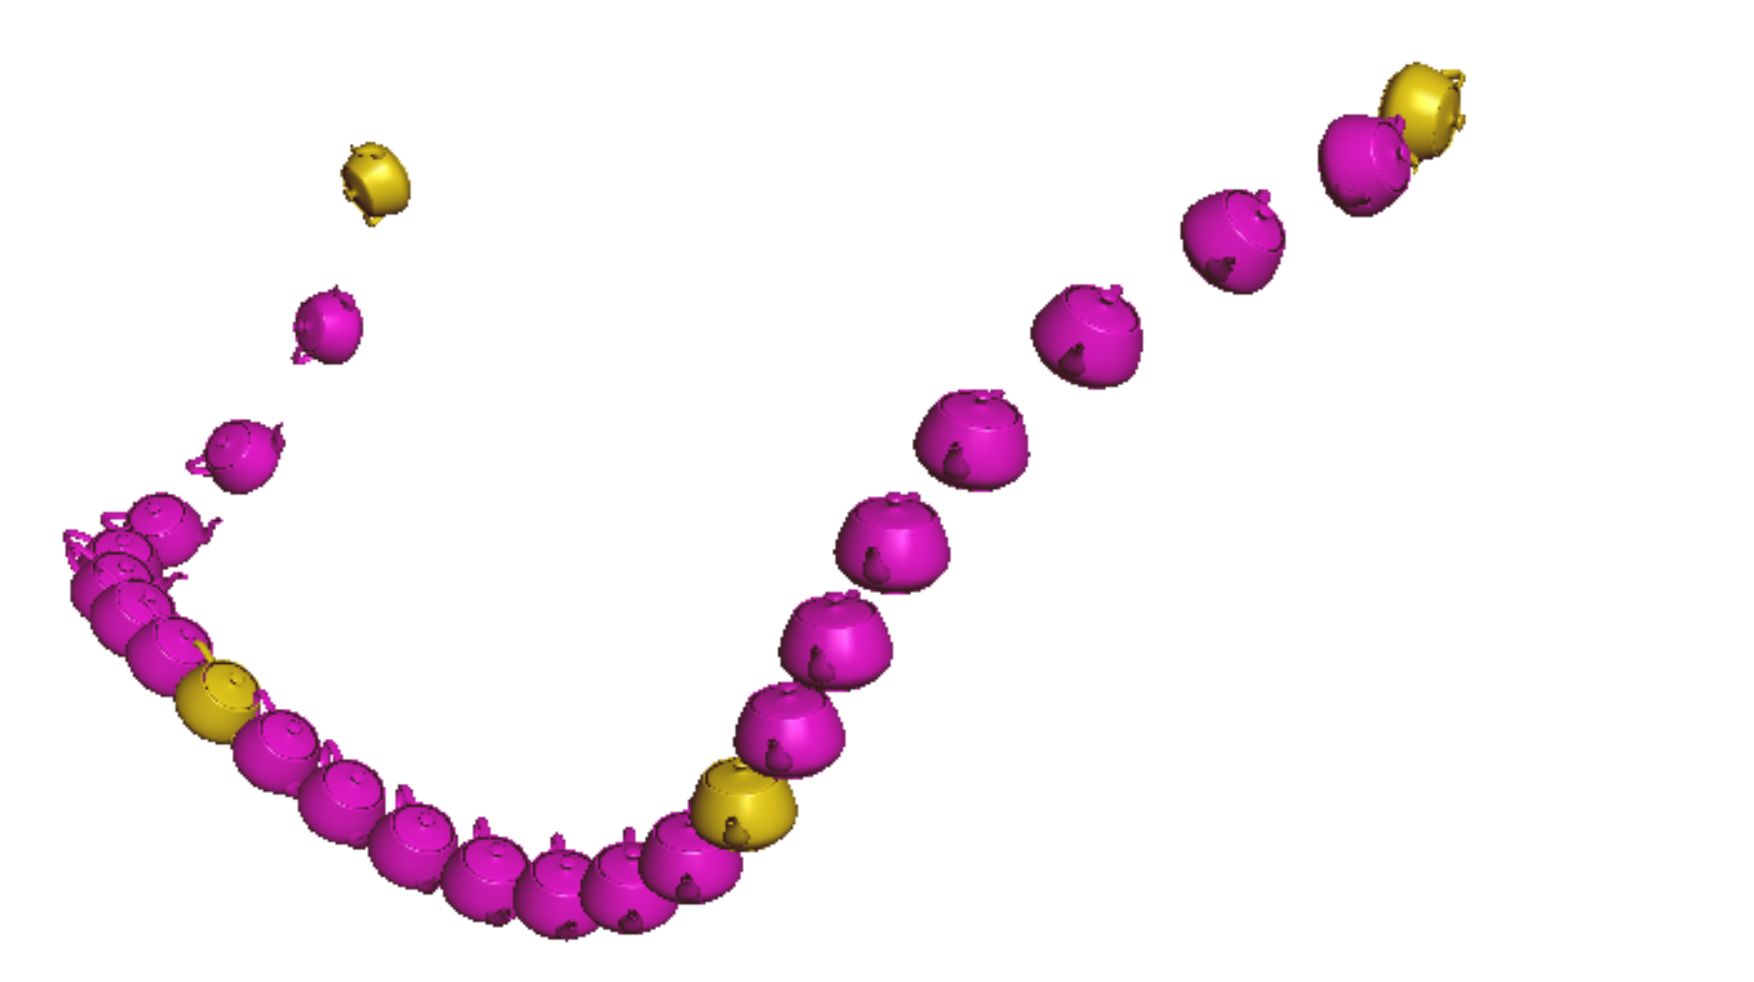
\includegraphics[width=0.75\textwidth]{DQ_B-spline.png}
  \caption{Degree 3 B-spline interpolation of dual quaternions.}
  \label{Figure: 2}
\end{figure}
\\
Let $N$ denote a matrix of the above basis functions, and now we begin to solve for the control points:
$$ P = (N^T N)^{-1}( N^TQ_i) \qquad i = 0,\ldots, n-1$$
Where $Q_i$ are the spatial descriptions of the points taken from the user input expressed as dual quaternions. Also noting that again the number of control points calculated for is reliant on the user input.
\\
\\
Now that we have calculated for our control points we can compute the resulting motion. We use the same basis function formulation $N_{i,p}$ as in the B-spline section with all the weights equal to 1.
$$ Q = \frac{\sum^n_{i=0} \omega_i P_i N_{i,p}(u)}{\sum^n_{i=0} \omega_i N_{i,p}(u)}$$
$Q$ is expressed as a dual quaternion. To generate the resulting motion, we convert the dual quaternion into a homogeneous matrix and output the result. Figure 2 is an example of when the number of control points is equal to the number of spatial displacements, which creates an interpolation curve. This specific curve shows a smooth third degree curve which flows nicely through the spatial displacements.
\\
\\
\textbf{\large{Interpolation/Approximation Using Polar Decomposition}}
\\
The polar decomposition method starts by taking the user inputs of the spatial descriptions of the points expressed as dual quaternions and converting them into a pair of quaternions commonly referred to as biquaternions, or double quaternions. We begin by solving for the individual quaternions $G$ and $H$:
$$ G = \frac{Q + \epsilon Q^0}{r} \qquad H = \frac{Q - \epsilon Q^0}{r}$$
$Q$ is the rotation quaternion and $Q^0$ is the quaternion derived from the translation vector. These are taken from the user input and the number of these components are dependant on the number of spatial displacements.
$$ \epsilon = \frac{1}{R} \qquad R = \frac{24L}{\pi} $$
$$ r = \frac{\sqrt{4R^2+d^2}}{2R} \qquad d = |t| $$
Where $t$ is the translation vector entered in by the user for each spatial displacement.
\\
\\
It is also important to note that the basis functions $N_{i,p}(\bar{u}_k)$ and $N_{i,p}(u)$, along with the knots and parameter values, are calculated exactly the same way as the previous method. We move on to calculating the control points in both the $G$ and $H$ space:
$$ P_G = (N^T N)^{-1}( N^TG_i) \qquad P_H = (N^T N)^{-1}( N^TH_i) $$
Where $i = 0,\ldots, n$; and the basis function $N$ and control points $P$ are dependant on the number of control points picked by the user. We also solve for the rational B-spline motion in the $G$ and $H$ space separately:
$$ Q_G = \frac{\sum^n_{i=0} \omega_i P_G N_{i,p}(u)}{\sum^n_{i=0} \omega_i N_{i,p}(u)} \qquad  Q_H = \frac{\sum^n_{i=0} \omega_i P_H N_{i,p}(u)}{\sum^n_{i=0} \omega_i N_{i,p}(u)}$$
To terminally solve for the interpolation/approximation we have to combine $G$ and $H$ and build a resulting dual quaternion:
$$Q_G+Q_H=DQ+D^*Q=(D+D^*)Q=2D_4Q$$
Because the rotational quaternion, $Q$, should be a unit quaternion, the previous equation then implies that $2D_4$ is the norm of the quaternion $Q_G+Q_H$.
$$ Q = \frac{Q_G + Q_H}{|Q_G + Q_H|} $$
$$ D4 = \frac{|Q_G + Q_H|}{2} \qquad r = \frac{1}{D4} $$
$$ rG=Q+\epsilon Q^0=Q+\frac{Q^0}{R}$$
$$ Q^0 = R(rQ_G-Q)$$
Where $Q^0$ is in the form of a quaternion.
$$ Q_{GH} = \{Q,Q^0\} $$
$Q_{GH}$ is the resulting transformation from spaces $G$ and $H$ being combined into a singular dual quaternion.
Similar to the previous method, we generate the resulting motion by converting the dual quaternion $Q_{QH}$ into a homogeneous matrix and outputting the result. Figure 3 illustrates an instance where the number of control points is one less than the number of spatial displacements. The result is an approximation curve rather a perfect interpolation.
\\
\begin{figure}[h]
  \centering
  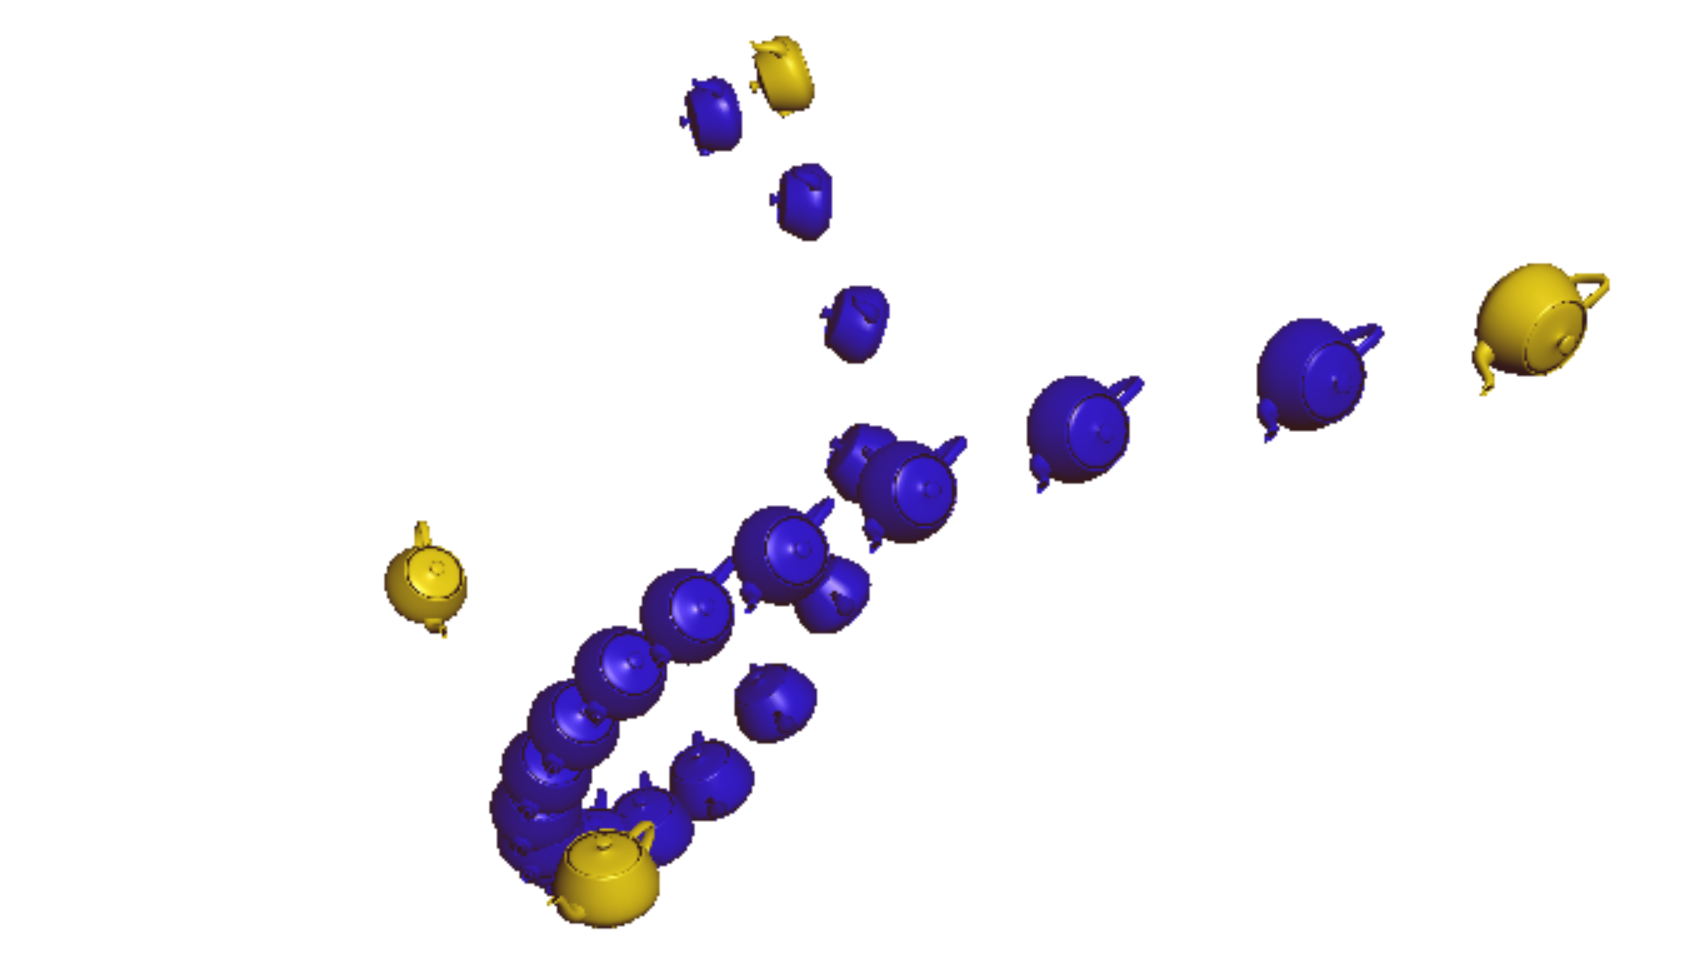
\includegraphics[width=0.75\textwidth]{Polar_Approx.png}
  \caption{Degree 2 B-spline approximation using 3 control points and polar decomposition method.}
  \label{Figure: 3}
\end{figure}
\\
\textbf{\large{Graphical User Interface}}
\\
The graphical user interface (GUI) enhances the user experience by optimizing the number of ways to manipulate a curve. Once our program is open, the user initially sees the "Input Filename:" in the top left corner. This allows the user to call on a file that describes the spatial descriptions of the displacements. An infinite amount of spatial descriptions is allowed but the characteristics have to be expressed as first, the rows of rotation quaternions and then the rows of translation (x,y,z,0). The name of a text input file must be entered manually, and therefore must known in advance. The input files themselves must be saved in the same folder as the program executable file. If a user attempts to upload a non-existent file, the console window will display an error message. The error can also be detected if the "Uploaded Data" checkbox does not generate the graphics for the input data in yellow.
\\
\\
Next we see a panel labeled as "Rational B-spline Motion". This is where our implementation can be applied by checking the respective boxes to obtain the desired curve. Through this panel, the data points can be used as control points to generate B-spline motion, or they can be used as spatial displacements for interpolation or approximation on either the dual quaternions themselves or their corresponding polar decompositions.
\\
\\
The controls present in our program are the degree, number of control points, resolution, and the hyperspherical radius. These controls are shown in Figure 4. The degree is an important control that is present in all the algorithms and tends to change the curve dramatically when altered. Because the same degree control is used for both the B-spline motion algorithm and the interpolation/approximation algorithm, the degree is limited to one less than the number of data points the user uploads. Higher order approximations could be possible if the user were to select a number of control points larger than the supplied number of data points. These scenarios were deemed computationally expensive and unnecessary, and as such are not handled in this implementation.
\\
\begin{figure}[h]
  \centering
  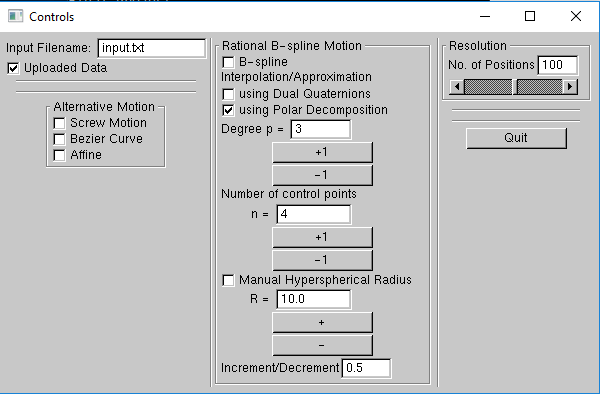
\includegraphics[width=0.75\textwidth]{GUI.png}
  \caption{The user interface that is coupled with our program. }\label{Figure: 4}
\end{figure}
\\
The number of control points is our way of manifesting the interpolation/approximation motion with precision control. If an individual desires an interpolation motion then the number of control points have to equal the number of spatial displacements the user has entered. An approximation motion can be achieved by having a number of control points less than the number of entered spatial displacements. A simpler curve can be witnessed if you continue to decrease the number of control points because there are less control points to define the motion path. The resolution can be changed with an integer slider ranging from 1 to 200. Increasing the resolution will result in more points between the spatial displacements.
\\
\\
A control was added to modify the hyperspherical radius, $R$, seen in the beginning steps of the polar decomposition algorithm. When the "Manual Hyperspherical Radius" box is unchecked, this value is calculated according to the alrogithm detailed above. When the box is checked however, a user can manually decide the setting for $R$ to view the effects this radius has on the resulting motion generation. Using this feature enables the user to see that the resulting polar decomposition interpolation approaches the dual quaternion interpolation in the limit as $R$ is increased. Figure 5 shows an example of this effect.
\\
\begin{figure}[h]
  \centering
  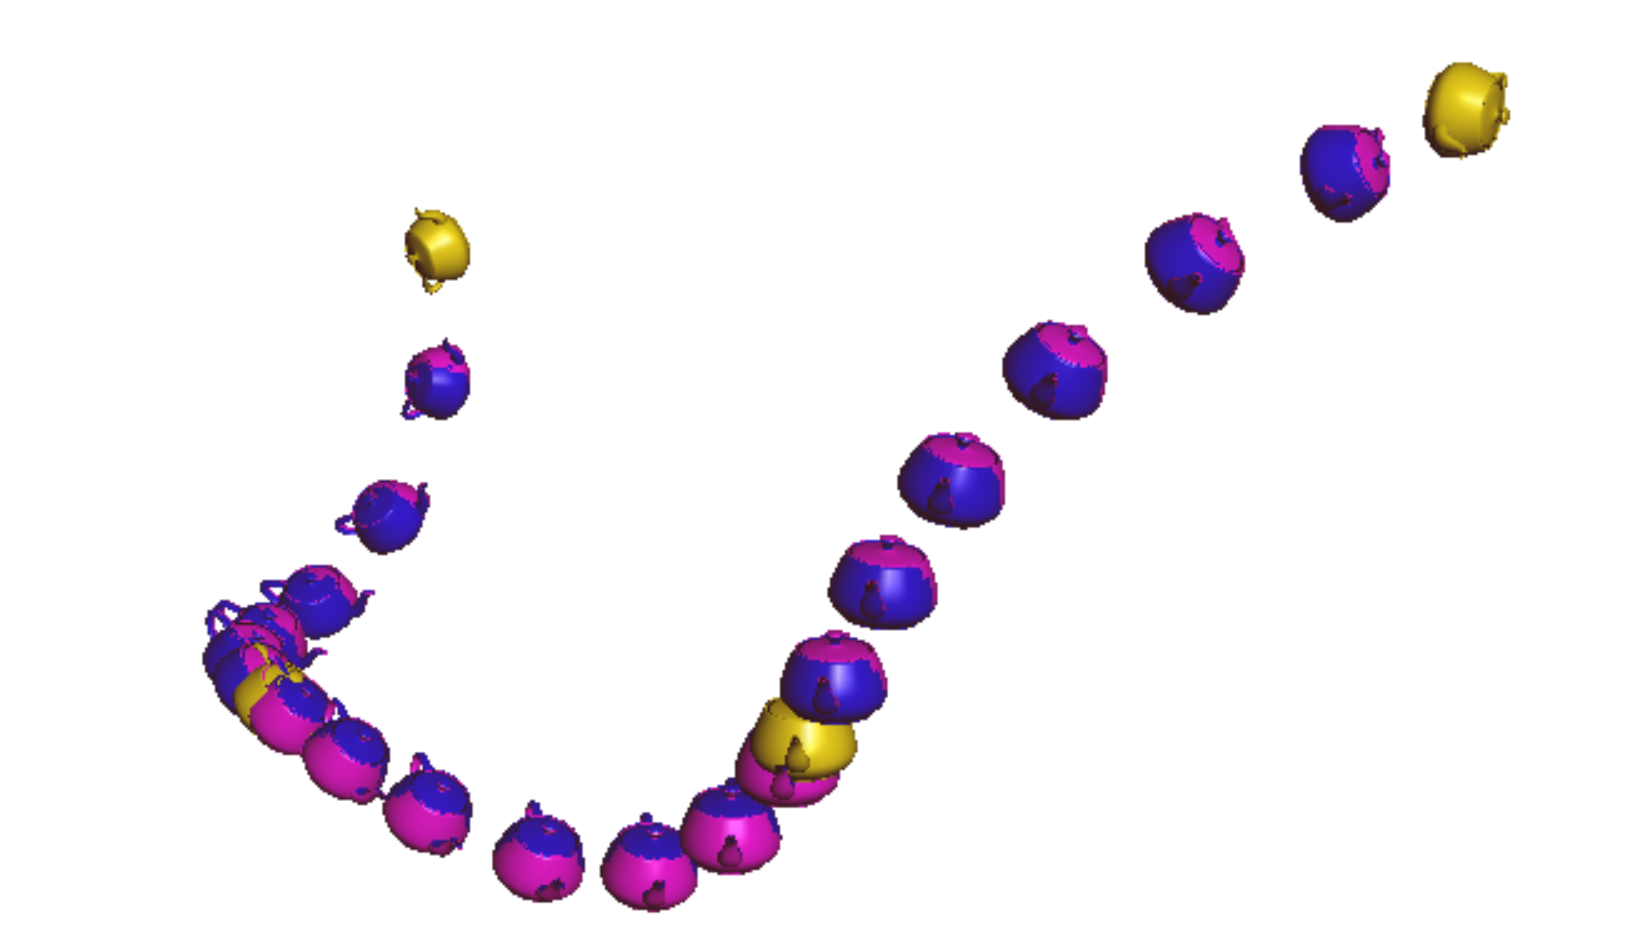
\includegraphics[width=0.75\textwidth]{Compare.png}
  \caption{Degree 2 B-spline interpolation using the dual quaternion (magenta) and polar decomposition (blue) methods. }
  \label{Figure: 5}
\end{figure}
\\
A default file containing 4 spatial displacements is included with the software to demonstrate the proper functionality of the program.

\newpage
\section{Conclusion}
This paper has developed algorithms for displaying motion using the rational B-spline curve. The three methods for generating this curve were interpolation, approximation and using the spatial displacements as control points. These methods allow the user a great sense of freedom for manipulating and designing a curve. Along with generating motion, this implementation demonstrated the role played by the approximating hyperspherical radius, $R$, in the polar decomposition of dual quaternions. Future upgrades to this software could include implementing user control over weights and knot vectors, which were decided to be secondary features for the purpose of this prototype. Various advanced features could also be added for motion smoothing or knot insertion for finer motion manipulation. Allowing a user to edit a position and orientation of an interpolation point directly in the interface would also be a useful feature. A fully featured implementation of this software could be useful in the fields of robotics and computer graphics.
\\
\\
\textbf{Acknowledgements:}
The authors would like to thank Anurag Purwar for the C++ skeleton code which included in depth quaternion and dual quaternion arithmetic along with various matrix operations.

\newpage
\textbf{References}
\begin{enumerate}
   \item Larochelle, P., and McCarthy, J. M., 1994, ``Designing Planar Mechanisms Using a Bi-Invariant Metric in the Image Space of SO(3),'' Proceedings of the 1994 ASME Design Engineering Technical Conferences, Vol. DE-70, ASME Press, pp.221-–228.
  \item Piegl, Les and Tiller, Wayne, 1995. The NURBS Book.
  \item Purwar, Anurag and Q. J. Ge., 2013, ``Polar Decomposition of Unit Dual Quaternions." Journal of Mechanisms and Robotics, vol. 5, no. 4, p. 041001.
\end{enumerate}
\end{document}
